\documentclass[12pt]{article}
\usepackage{graphicx}
\usepackage {color}
\usepackage{pdfpages}
\usepackage{float}
\usepackage{changebar}
\usepackage{enumitem,amssymb}
\renewcommand{\familydefault}{\sfdefault}
\usepackage[margin=1.2in]{geometry}
\usepackage{graphicx}
\usepackage{wrapfig}
\usepackage[super]{cite}
\usepackage{subcaption}
\usepackage[table]{xcolor}
\usepackage{amsmath}
\usepackage[sort, numbers]{natbib}

%%%%%%%%%%%%Defining the margins %%%%%%%%%%%%%%%%%%%%%
\textheight 9.in
\textwidth 6.5in
\topmargin -.5in
\oddsidemargin 0in
\setlength{\parskip}{\smallskipamount}

%%%%%%%%%%%%%%Specific Commands %%%%%%%%%%%%%%%%%%
\newcommand{\eg}{{\em e.g.,}}
\newcommand{\ie}{{\em i.e.,}}
\newcommand{\etc}{{\em etc.,}}
\newcommand{\etal}{{\em et al.}}
\newcommand{\degrees}{{$^{\circ}$}}
\newcommand{\micro}{{$\mu$}}


%%%%%%%%%%%%%%%%%%%%%%%%%%%% Setting to control figure placement
% These determine the rules used to place floating objects like figures 
% They are only guides, but read the manual to see the effect of each.
\renewcommand{\topfraction}{.9}
\renewcommand{\bottomfraction}{.9}
\renewcommand{\textfraction}{.1}
\renewcommand{\familydefault}{\sfdefault} %setting the san serif font

%%%%%%%%%%%%%%%%%%%%%%%% Line spacing
% Use the following command for ``double'' spacing
%\setlength{\baselineskip}{1.2\baselineskip}
% and this one for an acceptable NIH spacing of 6lpi based on 11pt
%\setlength{\baselineskip}{.9\baselineskip}
% The baselineskip does not appear to work when we include a maketitle
% command in the main file.  Something there must set the line spacing
% If we use this next command, then things seem to work.
\renewcommand{\baselinestretch}{.9}

\setcounter{secnumdepth}{0} %make no numbers but have a table of contents


\begin{document}

\title{Lab 4, Neuron and Backyard Brains}
\author{Jake Bergquist, u6010393}
\maketitle
\tableofcontents
\newpage

\section{Introduction}
In biology the study of structure and function relationships relies in part on various imaging techniques in order to assess the physical structure and layout of biological materials. At an organ and even to some extend a tissue level methods such as visible light microscopy cna be beneficial for resolving anatomical and cellular structure. However, when it comes to assessing biological specimens at a cellular and sub cellular level, higher resolution and finer detail are often required. Many of these methods of imaging of cellular level structures and organization rely on fluorescent labeling. This is a method by which specific substructures of a cell are tagged with material can be identified using florescent microscopy. The materials used to tag the cells are typically proteins conjugated to florescent molecules (in many cases a primary antibody protein attaches to the structure of interest and secondary antibody attaches to the primary antibody and carries the fluorescent molecule) or in some cases the fluorescent molecules themselves can act as specific or general tags. The targets of these tags range from specific proteins, protein subdomains, amino acid sequences, DNA, and other cellular components. Tissue samples are fixed and tagged using these various systems with several different fluorescent tags used simultaneously to assess multiple structures of interest within one tissue and there localization relative to one another. These fluorescent tags are visualized using fluorescent microscopy. This is a process by which the fluorescent molecules are induced to emit a wavelength of light which is specific to each fluorescent molecule. Each fluorescent molecule is characterized by an excitation and emission spectrum, which describes the wavelengths of light that will excite the electrons of the florescent molecule (the excitation spectrum), and what wavelength of light is released when the electrons fall back to their basal energy state (the emission spectrum). By shining light onto the specimen int he excitation spectrum and recording light from the emission spectrum the specific fluorescent molecules can be imaged. By adjusting the focus of the light shined onto and collected from the specimen down to a single point and scanning this point across the specimen and through its depth the 2D and 3D structure of the specimen can be resolved.

The specific tissue of interest in this report was taken from human atria. These tissue samples were labeled with wheat  germ  agglutinin (WGA)  conjugated  to  AlexaFluor-488 which stains the extracellular space and a stain for connexin43 (Cx43) with AlexaFluor-594. This allowed us to separately resolve the extracellular space which defines the spae of the cardiac myocytes as well as the spatial arrangement of the gap junctions (which contain two hexamers of connexin43/other connexins). Cardiac myocytes are typically cylindrical or ``brick" shaped cells that arrange into filaments and sheets.\cite{Woodcock2005} The gap junctions composed of two hexamers of connexins form open channels between cardiac myocytes. Gap junctions are found across the cell membrane where the myocytes is connected with its neighbor but the concentration is higher at the terminal ends of the myocytes.\cite{Mese2007} These gap junctions allow for free passage of ions and small molecules from cell to cell. This allows for the electrical activity of one cell such as the initiation of an action potential, to propagate to the neighboring cells. In this way the activating wavefront of cardiac electrical activity propagates from cell to cell in the heart. This leads to a synchronized and ordered wave of electrical activation across the heart which in turn leads to an ordered contraction of the heart.\cite{Mese2007} The arrangement of gap junctions throughout the cell plays a critical role in controlling the direction and propagation properties of this excitation wave. As such, visualizing the structure and arrangement of gap junctions in myocytes can be informative when examining disease states where gap junction remodeling is implicated.

\section{Methods}
\subsection{Image Acquisition}
Atrial tissue samples were obtained fromt he lab instructor. These samples had be prepared with WGA conjugated to AlexaFluor-488 stain and an anti-connexin43 antibody conjugated to AlexxaFluor-594. The sample was imaged using excitation spectra of | nm (for the WGA 488 fluorophore) and | nm (for the connexin 594 fluorophore). Recording were done with either the hybrid photomultiplier or the conventional photomultiplier. The effect of increasing laser power, changing photomultiplier gain, and changing pinhole size were examined. Additionally a 3D stack of images was acquired by sampling at 50 depths through the tissue.
\par{Baseline:} A baseline image was acquired with a pinhole size of 1 AU, 1024 x 1024 pixels (| \micro m pixel size), and lazer power of | and | for the | nm and |nm lasers respectively. The hybrid photomultiplier was used with default settings. Two images were take, one using the | nm filter and another with the |nm filter uin order to record signal from both fluorophores.
\par{Laser Power:} A 2D image was taken with increased laser power. The | nm laser power was increased from | to |, and the | nm laser was increased from | to |. All other parameters followed baseline parameters.
\par{Gain Adjustment:} A 2D image was acquired using the conventional photomultipliers with a gain of 500 V and 700 V. All other parameters followed the baseline parameters.
\par{Pinhole Size:} A 2D image was acquired with a pinhole size of 3 AU. All other parameters followed the baseline parameters.
\par{3D Stack: } A 3D stack was acquired at a resolution of 512 x 512 pixels per stack ( | \micro m pixel size). A total of 50 slices were taken making for a 512 x 512 x 50 image stack for both fluorophore channels. All other parameters followed the baseline parameters.

\subsection{Image Processing}
Fir each of the 2d images the .liff stack was imported to the FIJI processing system. Each image was manually adjusted for brightness and contrast to provide the clear visualization. Due to the requirements of the lab, each image was set at a constant relative scaling from 0 to 64\% of the intensity histogram when the brightness and constrast was adjusted. For each 2d image the histogram of signal intensities was assessed for the WGA channel. A threshold was applied at an intensity value of the mode plus one standard deviation. This threshold was used to make a selection in the image of the background signal. The histogram of this background was assessed to calculate the standard deviation of the background. The selection was then inverted to attain a selection of the signal. The histogram of the signal was used toc alculate the mean signal intensity, which when divided by the background standard deviation produced the signal to noise ratio (SNR) of the image. The WGA channel was visualized along with the total signal histogram for each parameter manipulation. Additionally the baseline image cas was visulized using a merged image of the WGA and CX43 channels, with the WGA chanel colored red and the cx43 channel colored green.


\section{Results}


\begin{figure}
	\begin{subfigure}{.5\textwidth}
		\centering
		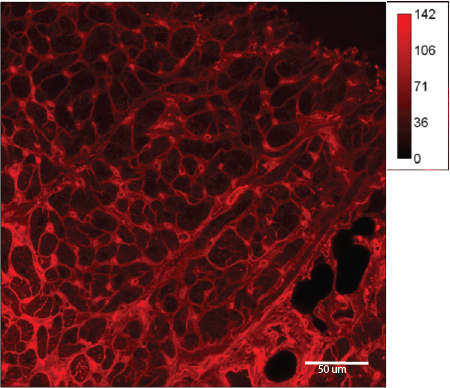
\includegraphics[width=.95\linewidth]{FinalFigures/WGA_Baseline.png}
		\caption{}
		\label{fig:wga_b}
	\end{subfigure}%
	\begin{subfigure}{.5\textwidth}
		\centering
		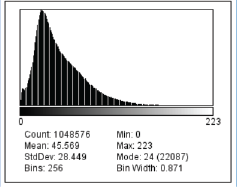
\includegraphics[width=.95\linewidth]{FinalFigures/WGA_Baseline_Hist.png}
		\caption{}
		\label{fig:wga_b_hist}
	\end{subfigure}
	\caption{Baseline WGA signal using baseline settings and the hybrid photomultiplier. The acquired signal is shown (a) in red with a 50 micron scale bar in the bottom right. The accompanying signal intensity histogram (b) shows a mode intensity fo 24 with standard deviation of 28.449.}
	\label{fig:wga_base}
\end{figure}


\begin{figure}
	\begin{subfigure}{.5\textwidth}
		\centering
		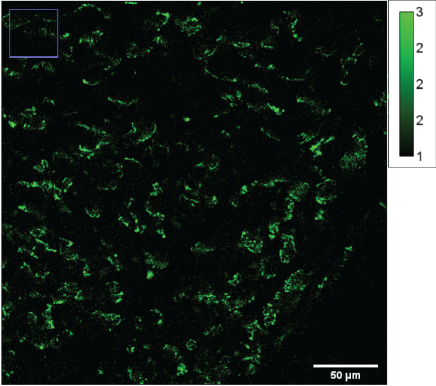
\includegraphics[width=.95\linewidth]{FinalFigures/CX43_Baseline.png}
		\caption{}
		\label{fig:cx43_b}
	\end{subfigure}%
	\begin{subfigure}{.5\textwidth}
		\centering
		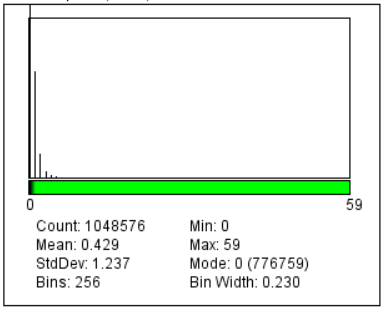
\includegraphics[width=.95\linewidth]{FinalFigures/CX43_baseline_Hist.png}
		\caption{}
		\label{fig:cx43_b_hist}
	\end{subfigure}
	\caption{Baseline connexin signal using baseline settings and the hybrid photomultiplier. The acquired signal is shown (a) in green with a 50 micron scale bar in the bottom right. The accompanying signal intensity histogram (b) shows a mode intensity fo 0 with standard deviation of 1.237.}
	\label{fig:cx43_base}
\end{figure}

\begin{figure}
	
		\centering
		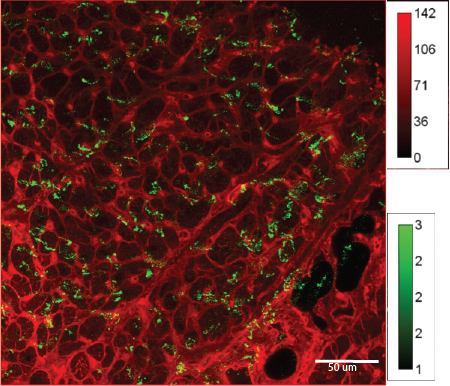
\includegraphics[width=.95\textwidth]{FinalFigures/BaselineMerge.png}
		
	\caption{Baseline connexin and WGA signal merged using baseline settings and the hybrid photomultiplier. The acquired signal is shown with connexin signal in green and WGA snal in red. A 50 micron scale bar is shown in the bottom right.}
	\label{fig:base_merge}
\end{figure}

\begin{figure}
	
	\centering
	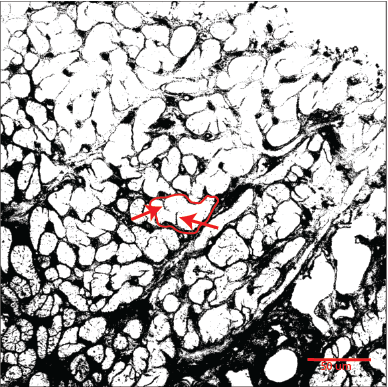
\includegraphics[width=.95\textwidth]{FinalFigures/WGA_Baseline_Binary.png}
	
	\caption{Baseline connexin and WGA signal merged using baseline settings and the hybrid photomultiplier. The acquired signal is shown with connexin signal in green and WGA snal in red. A 50 micron scale bar is shown in the bottom right.}
	\label{fig:base_binary}
\end{figure}

\begin{figure}
	\begin{subfigure}{.5\textwidth}
		\centering
		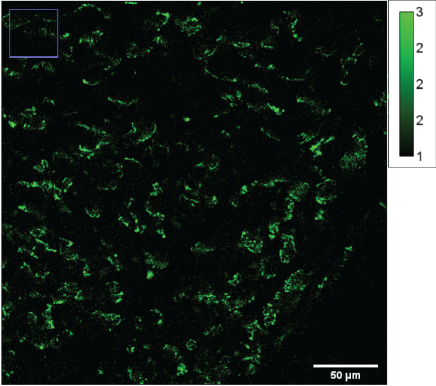
\includegraphics[width=.95\linewidth]{FinalFigures/CX43_Baseline.png}
		\caption{}
		\label{fig:cx43_b}
	\end{subfigure}%
	\begin{subfigure}{.5\textwidth}
		\centering
		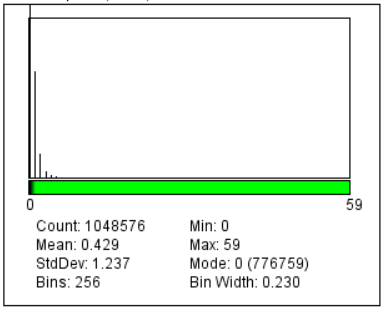
\includegraphics[width=.95\linewidth]{FinalFigures/CX43_baseline_Hist.png}
		\caption{}
		\label{fig:cx43_b_hist}
	\end{subfigure}
	\caption{Baseline connexin signal using baseline settings and the hybrid photomultiplier. The acquired signal is shown (a) in green with a 50 micron scale bar in the bottom right. The accompanying signal intensity histogram (b) shows a mode intensity fo 0 with standard deviation of 1.237.}
	\label{fig:cx43_base}
\end{figure}

%%%%%%%%%%%%%%%%%% Correct Bibliography Style

\bibliography{C:/Users/Jake/Documents/library}
\bibliographystyle{ieeetr}


\end{document}








